\documentclass{ximera}

%\usepackage{todonotes}

\newcommand{\todo}{}

\usepackage{esint} % for \oiint
\ifxake%%https://math.meta.stackexchange.com/questions/9973/how-do-you-render-a-closed-surface-double-integral
\renewcommand{\oiint}{{\large\bigcirc}\kern-1.56em\iint}
\fi


\graphicspath{
  {./}
  {ximeraTutorial/}
  {basicPhilosophy/}
  {functionsOfSeveralVariables/}
  {normalVectors/}
  {lagrangeMultipliers/}
  {vectorFields/}
  {greensTheorem/}
  {shapeOfThingsToCome/}
  {dotProducts/}
  {partialDerivativesAndTheGradientVector/}
  {../productAndQuotientRules/exercises/}
  {../normalVectors/exercisesParametricPlots/}
  {../continuityOfFunctionsOfSeveralVariables/exercises/}
  {../partialDerivativesAndTheGradientVector/exercises/}
  {../directionalDerivativeAndChainRule/exercises/}
  {../commonCoordinates/exercisesCylindricalCoordinates/}
  {../commonCoordinates/exercisesSphericalCoordinates/}
  {../greensTheorem/exercisesCurlAndLineIntegrals/}
  {../greensTheorem/exercisesDivergenceAndLineIntegrals/}
  {../shapeOfThingsToCome/exercisesDivergenceTheorem/}
  {../greensTheorem/}
  {../shapeOfThingsToCome/}
  {../separableDifferentialEquations/exercises/}
  {vectorFields/}
}

\newcommand{\mooculus}{\textsf{\textbf{MOOC}\textnormal{\textsf{ULUS}}}}

\usepackage{tkz-euclide}
\usepackage{tikz}
\usepackage{tikz-cd}
\usetikzlibrary{arrows}
\tikzset{>=stealth,commutative diagrams/.cd,
  arrow style=tikz,diagrams={>=stealth}} %% cool arrow head
\tikzset{shorten <>/.style={ shorten >=#1, shorten <=#1 } } %% allows shorter vectors

\usetikzlibrary{backgrounds} %% for boxes around graphs
\usetikzlibrary{shapes,positioning}  %% Clouds and stars
\usetikzlibrary{matrix} %% for matrix
\usepgfplotslibrary{polar} %% for polar plots
\usepgfplotslibrary{fillbetween} %% to shade area between curves in TikZ
%\usetkzobj{all}
\usepackage[makeroom]{cancel} %% for strike outs
%\usepackage{mathtools} %% for pretty underbrace % Breaks Ximera
%\usepackage{multicol}
\usepackage{pgffor} %% required for integral for loops



%% http://tex.stackexchange.com/questions/66490/drawing-a-tikz-arc-specifying-the-center
%% Draws beach ball
\tikzset{pics/carc/.style args={#1:#2:#3}{code={\draw[pic actions] (#1:#3) arc(#1:#2:#3);}}}



\usepackage{array}
\setlength{\extrarowheight}{+.1cm}
\newdimen\digitwidth
\settowidth\digitwidth{9}
\def\divrule#1#2{
\noalign{\moveright#1\digitwidth
\vbox{\hrule width#2\digitwidth}}}




% \newcommand{\RR}{\mathbb R}
% \newcommand{\R}{\mathbb R}
% \newcommand{\N}{\mathbb N}
% \newcommand{\Z}{\mathbb Z}

\newcommand{\sagemath}{\textsf{SageMath}}


%\renewcommand{\d}{\,d\!}
%\renewcommand{\d}{\mathop{}\!d}
%\newcommand{\dd}[2][]{\frac{\d #1}{\d #2}}
%\newcommand{\pp}[2][]{\frac{\partial #1}{\partial #2}}
% \renewcommand{\l}{\ell}
%\newcommand{\ddx}{\frac{d}{\d x}}

% \newcommand{\zeroOverZero}{\ensuremath{\boldsymbol{\tfrac{0}{0}}}}
%\newcommand{\inftyOverInfty}{\ensuremath{\boldsymbol{\tfrac{\infty}{\infty}}}}
%\newcommand{\zeroOverInfty}{\ensuremath{\boldsymbol{\tfrac{0}{\infty}}}}
%\newcommand{\zeroTimesInfty}{\ensuremath{\small\boldsymbol{0\cdot \infty}}}
%\newcommand{\inftyMinusInfty}{\ensuremath{\small\boldsymbol{\infty - \infty}}}
%\newcommand{\oneToInfty}{\ensuremath{\boldsymbol{1^\infty}}}
%\newcommand{\zeroToZero}{\ensuremath{\boldsymbol{0^0}}}
%\newcommand{\inftyToZero}{\ensuremath{\boldsymbol{\infty^0}}}



% \newcommand{\numOverZero}{\ensuremath{\boldsymbol{\tfrac{\#}{0}}}}
% \newcommand{\dfn}{\textbf}
% \newcommand{\unit}{\,\mathrm}
% \newcommand{\unit}{\mathop{}\!\mathrm}
% \newcommand{\eval}[1]{\bigg[ #1 \bigg]}
% \newcommand{\seq}[1]{\left( #1 \right)}
% \renewcommand{\epsilon}{\varepsilon}
% \renewcommand{\phi}{\varphi}


% \renewcommand{\iff}{\Leftrightarrow}

% \DeclareMathOperator{\arccot}{arccot}
% \DeclareMathOperator{\arcsec}{arcsec}
% \DeclareMathOperator{\arccsc}{arccsc}
% \DeclareMathOperator{\si}{Si}
% \DeclareMathOperator{\scal}{scal}
% \DeclareMathOperator{\sign}{sign}


%% \newcommand{\tightoverset}[2]{% for arrow vec
%%   \mathop{#2}\limits^{\vbox to -.5ex{\kern-0.75ex\hbox{$#1$}\vss}}}
% \newcommand{\arrowvec}[1]{{\overset{\rightharpoonup}{#1}}}
% \renewcommand{\vec}[1]{\arrowvec{\mathbf{#1}}}
% \renewcommand{\vec}[1]{{\overset{\boldsymbol{\rightharpoonup}}{\mathbf{#1}}}}

% \newcommand{\point}[1]{\left(#1\right)} %this allows \vector{ to be changed to \vector{ with a quick find and replace
% \newcommand{\pt}[1]{\mathbf{#1}} %this allows \vec{ to be changed to \vec{ with a quick find and replace
% \newcommand{\Lim}[2]{\lim_{\point{#1} \to \point{#2}}} %Bart, I changed this to point since I want to use it.  It runs through both of the exercise and exerciseE files in limits section, which is why it was in each document to start with.

% \DeclareMathOperator{\proj}{\mathbf{proj}}
% \newcommand{\veci}{{\boldsymbol{\hat{\imath}}}}
% \newcommand{\vecj}{{\boldsymbol{\hat{\jmath}}}}
% \newcommand{\veck}{{\boldsymbol{\hat{k}}}}
% \newcommand{\vecl}{\vec{\boldsymbol{\l}}}
% \newcommand{\uvec}[1]{\mathbf{\hat{#1}}}
% \newcommand{\utan}{\mathbf{\hat{t}}}
% \newcommand{\unormal}{\mathbf{\hat{n}}}
% \newcommand{\ubinormal}{\mathbf{\hat{b}}}

% \newcommand{\dotp}{\bullet}
% \newcommand{\cross}{\boldsymbol\times}
% \newcommand{\grad}{\boldsymbol\nabla}
% \newcommand{\divergence}{\grad\dotp}
% \newcommand{\curl}{\grad\cross}
%\DeclareMathOperator{\divergence}{divergence}
%\DeclareMathOperator{\curl}[1]{\grad\cross #1}
% \newcommand{\lto}{\mathop{\longrightarrow\,}\limits}

% \renewcommand{\bar}{\overline}

\colorlet{textColor}{black}
\colorlet{background}{white}
\colorlet{penColor}{blue!50!black} % Color of a curve in a plot
\colorlet{penColor2}{red!50!black}% Color of a curve in a plot
\colorlet{penColor3}{red!50!blue} % Color of a curve in a plot
\colorlet{penColor4}{green!50!black} % Color of a curve in a plot
\colorlet{penColor5}{orange!80!black} % Color of a curve in a plot
\colorlet{penColor6}{yellow!70!black} % Color of a curve in a plot
\colorlet{fill1}{penColor!20} % Color of fill in a plot
\colorlet{fill2}{penColor2!20} % Color of fill in a plot
\colorlet{fillp}{fill1} % Color of positive area
\colorlet{filln}{penColor2!20} % Color of negative area
\colorlet{fill3}{penColor3!20} % Fill
\colorlet{fill4}{penColor4!20} % Fill
\colorlet{fill5}{penColor5!20} % Fill
\colorlet{gridColor}{gray!50} % Color of grid in a plot

\newcommand{\surfaceColor}{violet}
\newcommand{\surfaceColorTwo}{redyellow}
\newcommand{\sliceColor}{greenyellow}




\pgfmathdeclarefunction{gauss}{2}{% gives gaussian
  \pgfmathparse{1/(#2*sqrt(2*pi))*exp(-((x-#1)^2)/(2*#2^2))}%
}


%%%%%%%%%%%%%
%% Vectors
%%%%%%%%%%%%%

%% Simple horiz vectors
\renewcommand{\vector}[1]{\left\langle #1\right\rangle}


%% %% Complex Horiz Vectors with angle brackets
%% \makeatletter
%% \renewcommand{\vector}[2][ , ]{\left\langle%
%%   \def\nextitem{\def\nextitem{#1}}%
%%   \@for \el:=#2\do{\nextitem\el}\right\rangle%
%% }
%% \makeatother

%% %% Vertical Vectors
%% \def\vector#1{\begin{bmatrix}\vecListA#1,,\end{bmatrix}}
%% \def\vecListA#1,{\if,#1,\else #1\cr \expandafter \vecListA \fi}

%%%%%%%%%%%%%
%% End of vectors
%%%%%%%%%%%%%

%\newcommand{\fullwidth}{}
%\newcommand{\normalwidth}{}



%% makes a snazzy t-chart for evaluating functions
%\newenvironment{tchart}{\rowcolors{2}{}{background!90!textColor}\array}{\endarray}

%%This is to help with formatting on future title pages.
\newenvironment{sectionOutcomes}{}{}



%% Flowchart stuff
%\tikzstyle{startstop} = [rectangle, rounded corners, minimum width=3cm, minimum height=1cm,text centered, draw=black]
%\tikzstyle{question} = [rectangle, minimum width=3cm, minimum height=1cm, text centered, draw=black]
%\tikzstyle{decision} = [trapezium, trapezium left angle=70, trapezium right angle=110, minimum width=3cm, minimum height=1cm, text centered, draw=black]
%\tikzstyle{question} = [rectangle, rounded corners, minimum width=3cm, minimum height=1cm,text centered, draw=black]
%\tikzstyle{process} = [rectangle, minimum width=3cm, minimum height=1cm, text centered, draw=black]
%\tikzstyle{decision} = [trapezium, trapezium left angle=70, trapezium right angle=110, minimum width=3cm, minimum height=1cm, text centered, draw=black]


\title{Analyzing}

\begin{document}

\begin{abstract}
describe everything
\end{abstract}
\maketitle




$\blacktriangleright$ \textbf{\textcolor{red!80!black}{Reasoning:}} Reasoning is a logical explanation that describes our conclusions, how we arrived at those conclusions, and why we think those conclusions are correct. \\

Analysis is not a list of conclusions. We are not looking for such a list. \\

We are looking for the thought process that arrived at the list of conclusions. \\




\begin{example}


\textbf{\textcolor{purple!85!blue}{Completely analyze}}

\[
p(k) = k \sqrt{4-k^2}
\]


with


\[
p'(k) = \sqrt{4-k^2} + k \frac{1}{2} \cdot (\sqrt{4-k^2})^{-\tfrac{1}{2}} \cdot (-2k)
\]

\begin{remark}

$p$ is not an elementary function.  It is a product of two functions. One of the factors is a linear funciton, $k$. \\

The other factor is not a linear function.  It is a composition of a root function and a quadratic function. \\

\end{remark}




$\blacktriangleright$  \textbf{\textcolor{blue!55!black}{Domain:}} 

The domain of a product is the intersection of the domains of the two factors. \\

The first factor is a linear function, so its domain is $(-\infty, \infty)$. \\

The second factor is a square root. We need the inside of the square root to be nonnegative (positive or zero).  So, we need $k^2 \leq 4$. That gives us $[-2, 2]$. \\




All together, the intersection leaves us with a natural domain of $[-2, 2]$ for $p$.





$\blacktriangleright$  \textbf{\textcolor{blue!55!black}{Continuity:}} 

Both $k$ and $\sqrt{4 - k^2}$ are continuous. \\


$k$ is a linear function. \\


The other factor is the composition of a square root and a quadratic. Both of those are continuous, which makes the second factor continuous. \\



$p$ is the product of continuous functions, so it is continuous.












$\blacktriangleright$  \textbf{\textcolor{blue!55!black}{Zeros:}} 


\[  p(k) = 0   \]

\[  k \sqrt{4-k^2} = 0  \]


By the Zero Product Property, we have that either $k = 0$ or $\sqrt{4-k^2} = 0$.


Zeros are $-2$, $0$, and $2$. \\








$\blacktriangleright$ \textbf{\textcolor{blue!55!black}{End-Behavior:}}  


End-behavior is only a feature of a function with a domain that is unbounded.  It the domain does not approach $-\infty$ or $\infty$, then there is no end-behavior.\\


Here, the domain is $[-2, 2]$.  So, there is no emdbehavior. \\













$\blacktriangleright$ \textbf{\textcolor{blue!55!black}{Behavior:}}  



We will use the derivative to decipher the behavior of $p$.  But first, let's see how far some algebraic thinking will get us. \\


\begin{idea}

Since $\sqrt{k^2 - 4} \geq 0$, the sign of $p(k)$ is the same as the sign of $\answer{k}$.

\begin{itemize}
\item  $p(k)$ \wordChoice{\choice[correct]{$<$} \choice{$>$}}  $0$ on $(-2, 0)$.
\item  $p(k)$ \wordChoice{\choice{$<$} \choice[correct]{$>$}}  $0$ on $(0, 2)$.
\end{itemize}


Since $p$ is continuous, we must have 


\begin{itemize}
\item  $p(-2) = 0$.
\item  We have $p(-2)=0$ and $p(k)<0$ on $(-2,0)$, therefore, $p(k)$ begins \wordChoice{\choice{increasing} \choice[correct]{decreasing}}  at $-2$.
\item  $p(k)$ eventually \wordChoice{\choice[correct]{increases} \choice{decreases}}  back to $p(0) = 0$.
\item  $p(k)$ continues \wordChoice{\choice[correct]{increasing} \choice{decreasing}}  beyond $p(0) = 0$.
\item  $p(k)$ eventually \wordChoice{\choice{increases} \choice[correct]{decreases}}  back to $p(2) = 0$.
\end{itemize}


There must be at least two critical numbers.  One inside $\left( \answer{-2}, \answer{0} \right)$ and one inside $\left( \answer{0}, \answer{2} \right)$.












Graph of $y = p(k)$.

\begin{image}
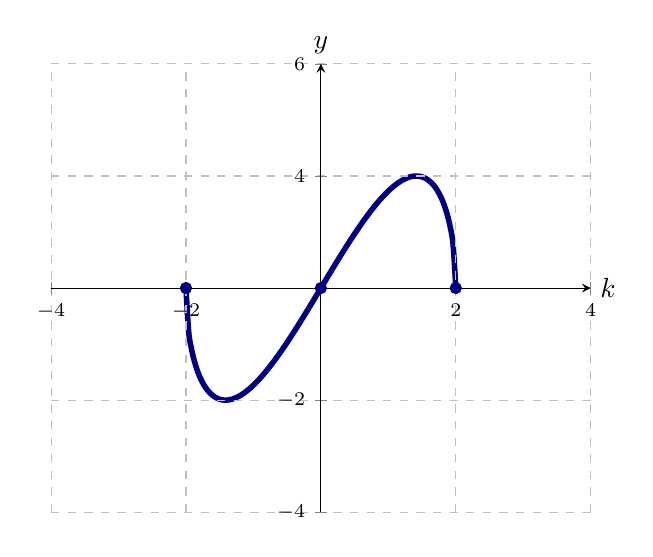
\begin{tikzpicture}
  \begin{axis}[
            domain=-2:2, ymax=4, xmax=4, ymin=-4, xmin=-4,
            axis lines =center, xlabel=$k$, ylabel={$y$}, grid = major, grid style={dashed},
            ytick={-4,-2,2,4},
            xtick={-4,-2,2,4},
            yticklabels={$-4$,$-2$,$4$,$6$}, 
            xticklabels={$-4$,$-2$,$2$,$4$},
            ticklabel style={font=\scriptsize},
            every axis y label/.style={at=(current axis.above origin),anchor=south},
            every axis x label/.style={at=(current axis.right of origin),anchor=west},
            axis on top
          ]
          

            %\addplot [line width=2, penColor, smooth,samples=100,domain=(-9:9)] {5/(1 + 3 * e^(-x/2))};
            \addplot [line width=2, penColor, smooth,samples=100,domain=(-2:2)] {x * sqrt(4 - x^2)};


            \addplot[color=penColor,fill=penColor,only marks,mark=*] coordinates{(-2,0) (0,0) (2,0)}; 





           

  \end{axis}
\end{tikzpicture}
\end{image}



With this thinking, we can make an algebraic approach \\


\end{idea}




We can use the sign of the derivative to help us figure out where $p$ increses and decreases, \\


Step #1 is finding the critical numbers. \\









$\blacktriangleright$ \textbf{\textcolor{blue!55!black}{Extrema:}}  


With a little help from DESMOS, we can \textbf{approximate} the critical numbers as $-1.414$ and $1.414$.



\begin{itemize}
\item  $p(k)$ decreasing on $[-2, -1.414]$.
\item  $p(k)$ increases on $[-1.414, 1.414]$.
\item  $p(k)$ decreases on $[1.414, 2]$.
\end{itemize}




$p(-1.414)$ is the approximate global (and local) minimum. \\

$p(1.414)$ is the approximate global (and local) maximum. \\



And this is the problem we face in Precalculus. We don't seem to have enough algebra tools to locate local minimums and maximums. Sometimes we can, depending on the formula, but mostly we cannot. We turn to graphs for help knowing that they might be hiding important information.\\



\end{example}













\section*{with Calculus}


Calculus will give us a formula for the derivative.

\[    p'(k) = \sqrt{4 - k^2} + k \cdot \frac{-2k}{\sqrt{4-k^2}}  \]


This derivative has zeros of $-\sqrt{2}$ and $\sqrt{2}$, which are approximately $-1.414$ and $1.4141$. 












\begin{center}
\textbf{\textcolor{green!50!black}{ooooo-=-=-=-ooOoo-=-=-=-ooooo}} \\

more examples can be found by following this link\\ \link[More Examples of Analyzing More Functions]{https://ximera.osu.edu/csccmathematics/precalculus2/precalculus2/analyzingMoreFunctions/examples/exampleList}

\end{center}





\end{document}
